\documentclass[10pt,compress]{beamer}
\usepackage{xspace}
\usepackage{tikz,pgfplots}
\usepackage{comment}

%\definecolor{blackish}{HTML}{23373B}

%% https://github.com/matze/mtheme.git
\usetheme{m}

\usepackage[lambda,landau,operators,probability,sets,logic,complexity,asymptotics]{cryptocode}

%
% UTF-8 all the things
% 
\usepackage{unicodesymbols} % put this after m which loads fontspec

\usepackage{amsmath,amsfonts,amssymb,amsthm}
\usepackage{xspace}
\usepackage{tikz}
\usepackage{graphicx}  % Required for including images
\usepackage{unicodesymbols}

\usetikzlibrary{calc}
\usetikzlibrary{arrows,automata}
\usetikzlibrary{positioning}

\definecolor{butter1}{rgb}{0.988,0.914,0.310}
\definecolor{chocolate1}{rgb}{0.914,0.725,0.431}
\definecolor{chameleon1}{rgb}{0.541,0.886,0.204}
\definecolor{skyblue1}{rgb}{0.447,0.624,0.812}
\definecolor{plum1}{rgb}{0.678,0.498,0.659}
\definecolor{scarletred1}{rgb}{0.937,0.161,0.161}

\newcommand{\vs}{\vspace{5mm}}

\newcommand{\lattice}[3] {
  \coordinate (anchor) at (#1);
  \coordinate (b1) at (#2);
  \coordinate (b2) at (#3);
,  \foreach \x in {0,1,2,3,4} {
    \foreach \y in {0,...,4} {
      \node [draw,circle,inner sep=1pt,fill] at ($(anchor) + {\x}*(b1) + {\y}*(b2)$) {};
    }
  }
}

\AtBeginSection[] {
  \begin{frame}
    \frametitle{Outline}
    \tableofcontents[sectionstyle=show/shaded,subsectionstyle=show/shaded]
  \end{frame}
}

\renewcommand{\vec}[1]{\mathbf{#1}\xspace}
\newcommand{\vol}[1]{\ensuremath{\textnormal{vol}\left(#1\right)}\xspace}

\newcommand{\A}{\vec{A}}
\newcommand{\s}{\vec{s}}
\newcommand{\ip}[2]{\left\langle{} {#1}, {#2} \right\rangle{}}
\newcommand{\Zq}{\ensuremath{\Z_q}\xspace}
\newcommand{\vectorbound}{\ensuremath{\kappa}}
\newcommand{\secretbound}{\ensuremath{\nu}}
\newcommand{\E}{\ensuremath{\textnormal{E}}}
\newcommand{\Var}{\ensuremath{\textnormal{Var}}}
\newcommand{\Udist}[1]{\ensuremath{\mathcal{U}(#1)\xspace}}
\newcommand{\dotp}[2]{\ensuremath{\left\langle {#1},{#2}\right\rangle}\xspace}
\newcommand{\pq}{\ensuremath{\frac{p}{q}}}
\renewcommand{\B}[2][]{\ensuremath{\mathcal{B}_{#1}^{#2}}\xspace}

\newcommand{\shortvec}[1]{\tilde{\mathbf{#1}}\xspace}
\renewcommand{\vec}[1]{\mathbf{#1}\xspace}
\newcommand{\chig}{\ensuremath{\chi_{\alpha,q}}}
\newcommand{\Z}{\ensuremath{\mathbb{Z}}\xspace}
\newcommand{\Zp}{\ensuremath{\mathbb{Z}_p}\xspace}
\newcommand{\Ldis}{L_{\mathbf{s},\chi}^{(n)}\xspace}
\renewcommand{\O}[1]{\ensuremath{{\mathcal{O}\left(#1\right)}}\xspace}
\newcommand{\round}[1]{\ensuremath{\left\lfloor{#1}\right\rceil}\xspace}
\newcommand{\Bdis}[1]{B_{\mathbf{s},\chi}{(b,#1,p)}\xspace{}}
\newcommand{\Bdissm}[1]{B_{small,\mathbf{s},\chi} (b,#1,p) \xspace}
\def\polyfactor{n\, \log_2^2 n}
\def\DAG{D_{{\rm AG}}}

\newcommand{\Ldisp}{\ensuremath{\mathcal{L}_{\s,χ,p}}\xspace}
\newcommand{\Q}[1][⋅]{\ensuremath{\mathcal{Q}_{\s}\left( {#1} \right)}\xspace}

\usepackage{listings}
\lstdefinelanguage{Sage}[]{Python}{morekeywords={True,False,sage,cdef,cpdef,ctypedef,self},sensitive=true}
\lstset{frame=none,
          showtabs=False,
          showspaces=False,
          showstringspaces=False,
          commentstyle={\color{mLightBrown}},
          keywordstyle={\color{mLightBrown}\textbf},
          stringstyle ={\color{mDarkBrown}},
          frame=single,
          language=Sage,
          basicstyle=\tt\tiny,
          backgroundcolor=\color{gray!190!black},
          }

%
% BibLaTeX
%

\usepackage[
    backend=bibtex,
    style=alphabetic,
]{biblatex}

\addbibresource{local.bib}
\addbibresource{abbrev3.bib}
\addbibresource{crypto_crossref.bib}

\DeclareFieldFormat{title}{\alert{#1}}
\DeclareFieldFormat[book]{title}{\alert{#1}}
\DeclareFieldFormat[inproceedings]{title}{\alert{#1}}
\DeclareFieldFormat[article]{title}{\alert{#1}}
\DeclareFieldFormat[misc]{title}{\alert{#1}}

\title{Some Remarks on Small Secret LWE}
\author[Martin R.\ Albrecht]{Martin R.\ Albrecht \texttt{@martinralbrecht}}
\institute{Information Security Group, Royal Holloway, University of London}
\date{Auckland, December 4, 2015}

\begin{document} 

\begin{frame}
  \maketitle
\end{frame}

\setcounter{tocdepth}{2}
\begin{frame}
  \frametitle{Outline}
  \tableofcontents
\end{frame}


\section{Introduction}

\begin{frame}{Learning With Errors}
  The Learning with Errors (LWE) problem was defined by Oded Regev~\footfullcite{STOC:Regev05}. 

  Given $(\vec{A},\vec{c})$ with $\vec{c} \in \Zq^{m}$, $\vec{A} \in \Zq^{m \times n}$, $\vec{s} \in \Zq^{n}$ and $\vec{e} \in \Zq^{m}$ do we have
  \[
    \left(\begin{array}{c}
            \\
            \\
            \\ 
            \vec{c} \\
            \\
            \\
            \\\end{array} 
        \right) = 
        \left(\begin{array}{ccc}
                \leftarrow & n & \rightarrow \\
                \\
                \\ 
                           & \vec{A} & \\
                \\
                \\
                \\
              \end{array} \right) 
            \times{}
            \left(\begin{array}{c}
                    \\ 
                    \vec{s} \\
                    \\
                  \end{array}\right) 
                + \left(\begin{array}{c}
                          \\
                          \\
                          \\ 
                          \vec{e} \\
                          \\
                          \\
                          \\
                        \end{array}\right)
  \]
  or $\vec{c} \sample \Udist{\Zq^{m}}$.
\end{frame}


\begin{frame}
  \frametitle{Parameters}

  \begin{columns}
    \column{.5\textwidth}
    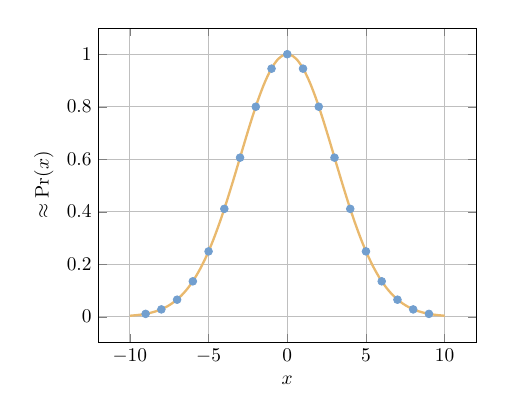
\begin{tikzpicture}[scale=0.7]
      \begin{axis}[
        domain=-10:10,
        grid=major,smooth,
        xlabel=$x$,
        ylabel=$\approx \textnormal{Pr}(x)$,
        ]
        \addplot[color=chocolate1,very thick,samples=50,smooth]{exp(-(x^2)/18)};
        \addplot[only marks,color=skyblue1] coordinates {
          (-9, 0.011)
          (-8, 0.028)
          (-7, 0.065)
          (-6, 0.135)
          (-5, 0.249)
          (-4, 0.411)
          (-3, 0.606)
          (-2, 0.800)
          (-1, 0.945)
          (0, 1.000)
          (1, 0.945)
          (2, 0.800)
          (3, 0.606)
          (4, 0.411)
          (5, 0.249)
          (6, 0.135)
          (7, 0.065)
          (8, 0.028)
          (9, 0.011)
        };
      \end{axis}
    \end{tikzpicture}
    \column{.50\textwidth}
    \begin{itemize}
    \item Parameters are: 
      \begin{itemize}
      \item dimension $n$, 
      \item modulus $q$,
      \item noise size $\alpha$,
       \item number of samples $m$.
      \end{itemize}

    \item Elements of $\vec{A}, \vec{s}, \vec{e}, \vec{c}$ are in $\mathbb{Z}_q$.
    \item $\vec{e}$ is sampled from a discrete Gaussian with width \[\sigma=\frac{\alpha q}{\sqrt{2 \pi}}.\]
    \end{itemize}
  \end{columns}
\end{frame}


\begin{frame}{LWE Normal Form}
  \begin{alertblock}{}
    Given samples \[(\vec{a},c)=(\vec{a},\langle\vec{a},\alert{\vec{s}}\rangle+ e) \in \Z_q^n \times \Z_q\] with $\vec{a} \gets \mathcal{U}(\Z_q^n)$, $e \gets D_{\alpha q,0}$ and $\vec{s} \in \Z_q^n$, we can construct samples \[(\vec{a}, c)=(\vec{a},\langle\vec{a},\alert{\vec{e}}\rangle+ e) \in \Z_q^n \times \Z_q\] 
    with $\vec{a} \gets \mathcal{U}(\Z_q^n)$, $e \gets D_{\alpha q, 0}$ and \alert{$\vec{e}$} such that all components \alert{$$e_i \gets D_{\alpha q, 0}$$} in polynomial time.\footfullcite{C:ACPS09}
  \end{alertblock}
\end{frame}

\begin{frame}{Small Secret LWE}
  \begin{itemize}
  \item Some applications use much smaller secrets.
  \item For example, $\vec{s}_{i} \leftarrow \{-1,0,1\}$ or $\vec{s_{i}} \leftarrow \{0,1\}$.
  \item {\tt HElib}\footfullcite{C:HalSho14} chooses $\vec{s}$ such that $h=64$ entries are $\pm 1$ and all remaining entries are $0$, regardless of dimension $n$.
  \end{itemize}

  \begin{block}{Question}
    How much security does this cost?
  \end{block}

\end{frame}


\begin{frame}{Hardness: Reductions}
  \begin{quote}
    ``A major part of our reduction [\dots] is therefore dedicated to showing  reduction from LWE (in dimension $n$) with arbitrary secret in $\Z_q^n$ to LWE (in dimension $n \log_2 q$) with a secret chosen uniformly over $\{0, 1\}$.''~\footfullcite{STOC:BLPRS13}
  \end{quote}
\end{frame}

\begin{frame}{Hardness: Algorithms}
  \begin{quote}
    ``[This work] suggests that this is overkill and that even $n\log\log n$ may be more than sufficient.''~\footfullcite{ACISP:BaiGal14}
  \end{quote}

\end{frame}

\begin{frame}{Hardness: Constructions}

  \begin{quote}
    ``This brings up the question of whether one can get better attacks against LWE instances with a very sparse secret (much smaller than even the noise). [\dots] it seems that the very sparse secret should only add maybe one bit to the modulus/noise ratio.''~\footfullcite{EPRINT:GenHalSma12}
  \end{quote}

\end{frame}


\begin{frame}{Binary LWE Secret Distributions}
  \begin{block}{}
    \begin{description}
    \item[$\B{+}$] each component is independently sampled uniformly from \(\{0,1\}\).
    \item[$\B{-}$] each component is independently sampled uniformly from \(\{-1,0,1\}\).  
    \item[$\mathcal{B}^{+}_{hw}$] like $\B{+}$ but with guarantee that  \(hw\) components are non-zero. 
    \item[$\mathcal{B}^{-}_{hw}$] like $\B{-}$ but with guarantee that  \(hw\) components are non-zero. 
    \end{description}
  \end{block}
\end{frame}


\begin{frame}{Lattice Reduction}

  In the guestimates below, we assumed
  \begin{itemize}
  \item $\delta_0 \approx {\left( \frac{k}{2 \pi e} {(\pi k)}^{\frac{1}{k}}  \right)}^{\frac{1}{2(k-1)}}$;
  \item the SVP oracle in BKZ is realise using sieving;
  \item sieving in blocksize $k$ costs $t_k = 2^{0.3366\,k + 12.31}$ clock cycles;
  \item BKZ-$k$ costs $\frac{n^3}{k^2} \log(n) \cdot t_k$ clock cycles in dimension $n$.
  \end{itemize}

  \begin{center}
    \url{https://github.com/dstehle/fplll}\\
     \url{https://github.com/malb/fpylll}   
  \end{center}

\end{frame}


\begin{frame}{Rolling Example}

We use the following LWE parameters as a rolling example throughout this talk.

  \begin{itemize}
  \item dimension $n=2048$,
  \item modulus $q ≈ 2^{63.4}$,
  \item noise parameter $\alpha ≈ 2^{-60.4}$, i.e.\ standard deviation $σ ≈ 3.2$,
  \item $h=64$ components of the secret are $\pm 1$, all other components are zero, $σ_s ≈ 0.44$: $\B[64]{-}$
  \end{itemize}

This is inspired by parameters chosen in {\tt HElib}.
  
\end{frame}

\section{Warm Up}

\begin{frame}{Exhaustive Search}
  
  \begin{itemize}
  \item Clearly, exhaustive search is an option for solving.
  \item This gives a complexity of about $2^n$ for $\B{+}$ and $3^n$ for $\B{-}$.
  \item For $\B[64]{-}$ we get a complexity of about $2^{64} ⋅ \binom{n}{64}$.
  \end{itemize}

  \begin{block}{Meet in the Middle}
    We can about square-root these complexities using standard time-memory trade-offs.
  \end{block}

  \begin{exampleblock}{HElib}
    Plugging our example in gives expected costs of $≈ 2^{470}$ and $≈ 2^{235}$ operations, respectively.    
  \end{exampleblock}

\end{frame}

\begin{frame}{Standard Approaches}

  Given $\vec{A},\vec{c}$ with $\vec{c} = \vec{A} \times \vec{s} + \vec{e}$ or $\vec{c} \sample \U{\Zq^m}$

  \begin{itemize}

  \item Solve the \alert{Short Integer Solutions} problem (SIS) in the left kernel of $\vec{A}$, i.e.
    \[
      \textnormal{ find a short } \vec{w} \textnormal{ such that } \vec{w} \times \vec{A} = 0
    \]
    and check if $\dotp{\vec{w}}{\vec{c}} = \vec{w}\times \left(\vec{A} \times \vec{s} + \vec{e}\right) = \dotp{\vec{w}}{\vec{e}}$ is short.
    \pause{}

  \item Solve the \alert{Bounded Distance Decoding} problem (BDD), i.e.\ 
    \[
      \textnormal{ find } \vec{s'} \textnormal{ such that } \abs{\vec{w} - \vec{c}} \textnormal{ with } \vec{w} = \vec{A} \times \vec{s'} \textnormal{ is minimised} .
    \]
    via Kannan's embedding or Babai's nearest planes.


  \end{itemize}
  
\end{frame}


\begin{frame}[fragile]{Standard Approaches vs.\ Rolling Example}
  \centering
  \begin{tikzpicture}[scale=0.95]
    \begin{axis}[
      legend pos=outer north east,
      axis lines=middle,
      xmin=0, xmax=4,
      ymin=0, ymax=160,
      axis y line*=left,
      axis x line*=bottom,
      xticklabels={SIS, DEC, Kannan}, 
      xtick={1,...,4},
      ytick={50,100,137.6,200},
      x tick label style={rotate=45,anchor=east},
      legend columns=1,
      legend cell align=left,]
      \addplot [only marks,color=skyblue1] table {
        1 142.6
        2 137.6
        3 138.8
      };
      \addplot[color=lightgray] table {
        0 137.6
        4 137.6
      };

    \end{axis}
  \end{tikzpicture}
  
\end{frame}


\section{Modulus Switching}

\begin{frame}{Modulus Switching}
  \begin{alertblock}{}
    Let $(\vec{a},c) =(\vec{a}, \langle \vec{a}, \vec{s} \rangle + e) \in \Z_q^n \times \Z_q$ be an LWE sample and \[p \approx \sqrt{\frac{2\pi\, n}{12}} \cdot \frac{\sigma_s}{\alpha},\] where $\sigma_s$ is the standard deviation of components of the secret $\vec{s}$. If $p<q$ then $$\bigg(\round{\pq \cdot \vec{a}}, \round{\pq \cdot  c}\bigg) \textnormal{ in } \Z_{\alert{p}}^n \times \Z_{\alert{p}}$$ follows a distribution close to an LWE distribution with $n, \sqrt{2}\alpha, \alert{p}$.
  \end{alertblock}

%   \framebreak{}

%   \begin{eqnarray*}
%     \round{\pq ⋅ c} &=& \round{\pq \bigg( \ip{\vec{a}}{\vec{s}} + e \bigg)}\\
%                     &=& \round{ \ip{\pq⋅\vec{a}}{\vec{s} } + \pq · e}\\
%                     &=& \round{ \ip{ \round{\pq⋅\vec{a} }}{\vec{s}} + \ip{\pq ⋅\vec{a} - \round{\pq⋅\vec{a}}}{\vec{s}} + \pq ⋅ e}\\
%                     &=& \ip{ \round{\pq ⋅\vec{a}}}{\vec{s}} + \ip{\pq ⋅\vec{a} - \round{\pq⋅\vec{a} }}{\vec{s}} + \pq·e+e' \\
%                     &=& \ip{ \round{ \pq ⋅ \vec{a} }}{\vec{s} }_{p} + e'' + \pq ⋅ e + e'
% \end{eqnarray*}
% where $e'$ is distributed in $\left(-0.5,0.5\right]$ and $e''$ is an inner product of small  $n$-dimensional vectors. 

  % \framebreak{}

  % Targeting $e'' \approx \pq⋅e$, i.e.\ that the standard deviations of both distributions are the same, we get
  % \begin{eqnarray*}
  %   \alpha\, p /\sqrt{2\pi}  & \approx& \sqrt{n/12}\, σ_s\\
  %   p &\approx& \sqrt{\frac{2\pi\, n}{12}} ⋅ \frac{σ_s}{\alpha}.\\
  % \end{eqnarray*}

  \fullcite{FOCS:BraVai11}

\end{frame}

\begin{frame}[allowframebreaks]{Slightly Better Modulus Switching for Cryptanalysis}

  \begin{itemize}
  \item We usually simply assume that the rounding noise is also some Gaussian distribution.
  \item However, the rounding noise is not completely out of our control.
  \item We know one component that goes into making it: \[\pq ⋅\vec{a} - \round{\pq⋅\vec{a} }\]
  \end{itemize}

  \framebreak{}
  
  Given known vectors $\vec{r}_i \sample {\left(-\frac{1}{2},\frac{1}{2}\right]}^n$ and an unknown fixed vector $\vec{s} \sample \B{}$, we call $\Q[\vec{r}_i]$ the distribution obtained by outputting $\round{\ip{\vec{r}_i}{\vec{s}}}$. %chktex 9

  \[ \Q[\pq ⋅\vec{a} - \round{\pq⋅\vec{a} }] = \ip{\pq ⋅\vec{a} - \round{\pq⋅\vec{a} }}{\vec{s}}_p +e'\]

  \framebreak{}

  Let $\vec{s} \sample \B{+}$. Let $\vec{r}_i = \pq ⋅ \vec{a}_i - \round{ \pq ⋅ \vec{a}_i}$. Let ${\Ldis}''$ be a distribution which outputs those $(\vec{a}_i', c_i')$ where $\sum{\vec{r}_i'} ≤ c⋅σ$ with $σ$ the standard deviation of $\Q[\vec{r}_i]$. 

  \vspace{1em}

  Then, $\Q[\vec{r}_i']$ for $\vec{r}_i' = \pq ⋅ \vec{a}_i' - \round{ \pq ⋅ \vec{a}_i'}$ satisfies:
  \[\prob{\Q[\vec{r}_i'] > C⋅σ} ≤  \frac{\exp\left(-C^2 + c\,C - c^2/2\right)}{2\,\pi ⋅ \left(C^2 - c\,C\right)}.\]

  Compare:
  \[\prob{\Q[\vec{r}_i] > C ⋅ σ} ≤ \frac{\exp\left({-C^2/2}\right)}{C \sqrt{2 π}}.\]

  % \framebreak{}

  % We define $x_i, y_i, z_i$ and write
  % \begin{eqnarray*}
  %   \sum_{j=0}^{n-1} {(\vec{r}_i)}_{(j)} 
  %   &=& \sum_{j\, |\, \vec{s}_j≠0}{(\vec{r}_i)}_{(j)}
  %       + \sum_{j\ \mid\, \vec{s}_j=0}{(\vec{r}_i)}_{(j)},\\
  %   z_i    &=& x_i + y_i.\\
  % \end{eqnarray*}

  % \vspace{-3em}

  % We have
  % \[\prob{x_i > C⋅σ \Big\vert\; z_i < c⋅σ} = \prob{x_i > C⋅σ} ⋅ \prob{y_i < c⋅σ-C⋅σ}.\]
  % Applying tail bounds we get:
  % \begin{eqnarray*}
  %   \prob{x_i > C⋅σ \Big\vert\; z_i < c⋅σ}
  %   &≤& \frac{\exp(-C^2/2)}{\sqrt{2π}\,C}  ⋅ \frac{\exp\left(-(c-C)^2/2\right)}{\sqrt{2π}\,(C-c)}\\ %chktex 3
  %   &=& \frac{\exp\left(-C^2 + c\,C - c^2/2\right)}{2\,\pi ⋅ \left(C^2 - c\,C\right)}.
  % \end{eqnarray*}
  % \vspace{-3em}

\end{frame}


\begin{frame}[allowframebreaks,fragile]{Modulus Switching + Lattice Reduction}

\vspace{-0.9em}
Applied to our rolling example:

\begin{center}
    \begin{tikzpicture}[scale=0.8]
    \begin{axis}[
      legend pos=outer north east,
      axis lines=middle,
      xmin=0, xmax=4,
      ymin=0, ymax=160,
      axis y line*=left,
      axis x line*=bottom,
      xticklabels={SIS, DEC, Kannan}, 
      xtick={1,...,4},
      ytick={50,100,137.6},
      x tick label style={rotate=45,anchor=east},
      legend columns=1,
      legend cell align=left,]
      \addplot [only marks,color=skyblue1] table {
        1 142.6
        2 137.6
        3 138.8
      };
      \addplot[color=lightgray] table {
        0 137.6
        4 137.6
      };
      \legend{no mod.\ switch}\;
    \end{axis}
  \end{tikzpicture}
\end{center}

\framebreak{}

Applied to our rolling example:

\begin{center}
  \begin{tikzpicture}[scale=0.8]
    \begin{axis}[
      legend pos=outer north east,
      axis lines=middle,
      xmin=0, xmax=4,
      ymin=0, ymax=160,
      axis y line*=left,
      axis x line*=bottom,
      xticklabels={SIS, DEC, Kannan}, 
      xtick={1,...,4},
      ytick={50,100,137.6,200},
      x tick label style={rotate=45,anchor=east},
      legend columns=1,
      legend cell align=left,]
      \addplot [only marks,color=skyblue1] table {
        1 142.6
        2 137.6
        3 138.8
      };
      \addplot [only marks,color=chocolate1] table {
        1 143.7
        2 138.7
        3 140.1
      };
      \addplot[color=lightgray] table {
        0 137.6
        4 137.6
      };
      \legend{no mod.\ switch, mod.\ switch}\;
    \end{axis}
  \end{tikzpicture}
\end{center}

\end{frame}

\subsection{Coded-BKW}

\begin{frame}[allowframebreaks,fragile]{BKW Algorithm}

The BKW algorithm was first proposed for the Learning Parity with Noise (LPN) problem which can be viewed as a special case of LWE over $\Z_{2}$.

\framebreak{}

We considering $a \approx \log n$ `blocks' of $b$ elements each.

\begin{equation*}
\left(\begin{array}{cc|ccc|c}
\bold{a}_{11} & \bold{a}_{12} & \bold{a}_{13} & \cdots & \bold{a}_{1n} & c_0\\
\bold{a}_{21} & \bold{a}_{22} & \bold{a}_{23} & \cdots & \bold{a}_{2n} & c_1\\
\vdots & \vdots & \ddots & \vdots & \vdots\\
\bold{a}_{m1} & \bold{a}_{m2} & \bold{a}_{m3} & \cdots & \bold{a}_{mn} & c_{m}
\end{array}\right)
\end{equation*}

\framebreak{}

For each block we build a table of all $q^b$ possible values indexed by $\Z_q^b$.

\begin{equation*}
T^0 = \left[ 
\begin{array}{ll|ccc|c}
-\lfloor\frac{q}{2}\rfloor & -\lfloor\frac{q}{2}\rfloor & \bold{t}_{13} & \cdots & \bold{t}_{1n} & c_{t,0}\\
-\lfloor\frac{q}{2}\rfloor & -\lfloor\frac{q}{2}\rfloor+1 & \bold{t}_{23} & \cdots & \bold{t}_{2n} & c_{t,1}\\
\phantom{--}\vdots & \phantom{--}\vdots & \ddots & \vdots & \vdots\\
\phantom{-}\lfloor\frac{q}{2}\rfloor & \phantom{-}\lfloor\frac{q}{2}\rfloor& \bold{t}_{q^23} & \cdots & \bold{t}_{q^2n} & c_{t,q^2}
\end{array}\right]
\end{equation*}

For each $\vec{z} \in \Z_q^b$ we try to find a row in $\vec{A}$ such that it contains $\vec{z}$ as a subvector at the target indices.

\framebreak{}

We use these tables to eliminate $b$ entries in other rows. Assume $(\vec{a}_{21},\vec{a}_{22}) = (\lfloor\frac{q}{2}\rfloor, \lfloor\frac{q}{2}\rfloor+1)$, then:
\begin{footnotesize}
\begin{eqnarray*}
& & \left(
\begin{array}{cc|ccc|c}
\vec{a}_{11} & \vec{a}_{12} & \vec{a}_{13} & \cdots & \vec{a}_{1n} & c_0\\
\alert{\vec{a}_{21}} & \alert{\vec{a}_{22}} & \vec{a}_{23} & \cdots & \vec{a}_{2n} & c_1\\
\vdots & \vdots & \ddots & \vdots & \vdots\\
\vec{a}_{m1} & \vec{a}_{m2} & \vec{a}_{m3} & \cdots & \vec{a}_{mn} & c_{m}
\end{array}
\right)\\
&+& \left[
\begin{array}{ll|ccc|c}
-\lfloor\frac{q}{2}\rfloor & -\lfloor\frac{q}{2}\rfloor & \bold{t}_{13} & \cdots & \bold{t}_{1n} & c_{t,0}\\
\alert{-\lfloor\frac{q}{2}\rfloor} & \alert{-\lfloor\frac{q}{2}\rfloor+1} & \bold{t}_{23} & \cdots & \bold{t}_{2n} & c_{t,1}\\
\phantom{--}\vdots & \phantom{--}\vdots & \ddots & \vdots & \vdots\\
\phantom{-}\lfloor\frac{q}{2}\rfloor & \phantom{-}\lfloor\frac{q}{2}\rfloor& \bold{t}_{q^23} & \cdots & \bold{t}_{q^2n} & c_{t,q^2}
\end{array}\right]\\
&\Rightarrow& \left(
\begin{array}{cc|ccc|c}
\vec{a}_{11} & \vec{a}_{12} & \vec{a}_{13} & \cdots & \vec{a}_{1n} & c_0\\
\alert{0} & \alert{0} & \shortvec{a}_{23} & \cdots & \shortvec{a}_{2n} & \tilde{c}_1\\
\vdots & \vdots & \ddots & \vdots & \vdots\\
\vec{a}_{m1} & \vec{a}_{m2} & \vec{a}_{m3} & \cdots & \vec{a}_{mn} & c_{m}
\end{array}
\right)\phantom{\Longrightarrow}
\end{eqnarray*}
 \end{footnotesize}
\end{frame}

\newcommand{\pivot}[4]{
\draw[fill=skyblue1]   (#1, #2) --(#1, #2+.5) -- (7.5, #2+.5) -- (7.5, #2) -- (#1, #2);
\draw[fill=skyblue1] (#3+0.5, #2) --(#3+0,   #2+.5) -- (7.5, #2+.5) -- (7.5, #2) -- (#3+0.5, #2);
\draw[fill=#4] (0,#2) -- (#1,#2) -- (#1,#2+.5) -- (0,#2+.5) -- (0,#2);
}

\begin{frame}[fragile]{Lazy Modulus Switching} 

% For simplicity assume $p = 2^\kappa$ and consider the LWE matrix
% \begin{eqnarray*}
% [\vec{A} \mid \vec{c}] &=& \left(\begin{array}{ccccc}
%        \vec{a}_{1,1} & \vec{a}_{1,2} & \hspace{2em} \cdots \hspace{2em} & \vec{a}_{1,n} & c_1\\
%        \vec{a}_{2,1} & \vec{a}_{2,2} & \cdots & \vec{a}_{2,n} & c_2\\
%         \vdots & \vdots & \ddots & \vdots & \vdots\\
%        \vec{a}_{m,1} & \vec{a}_{m,2} & \cdots & \vec{a}_{m,n} & c_{m}\\
%       \end{array}\right)\\
% \end{eqnarray*}
% as
% \begin{eqnarray*}
% [\vec{A} \mid \vec{c}] & = & \left(\begin{array}{cccccccc}
%        \vec{a}_{1,1}^h & \vec{a}_{1,1}^{l} \hspace{1em} & \vec{a}_{1,2}^h & \vec{a}_{1,2}^{l} & \hspace{1em} \cdots \hspace{1em} & \vec{a}_{1,n}^h & \vec{a}_{1,n}^{l}  \hspace{1em} & c_1\\
%        \vec{a}_{2,1}^h & \vec{a}_{2,1}^{l} \hspace{1em} & \vec{a}_{2,2}^h & \vec{a}_{2,2}^{l} & \hspace{1em} \cdots \hspace{1em} & \vec{a}_{2,n}^h & \vec{a}_{2,n}^{l}  \hspace{1em} & c_2\\
%         \vdots & \vdots & \vdots & \vdots & \ddots & \vdots & \vdots & \vdots\\
%        \vec{a}_{m,1}^h & \vec{a}_{m,1}^{l} \hspace{1em} & \vec{a}_{m,2}^h & \vec{a}_{m,2}^{l} & \hspace{1em} \cdots \hspace{1em} & \vec{a}_{m,n}^h & \vec{a}_{m,n}^{l}  \hspace{1em} & c_{m}\\
%       \end{array}\right)\\
% \end{eqnarray*}
% where $\vec{a}_{i,j}^h$ and $\vec{a}_{i,j}^{l}$ denote high and low order bits:
% \begin{itemize}
%  \item $\vec{a}_{i,j}^h$ corresponds to $\round{p/q \cdot \vec{a}_{i,j}}$ and 
%  \item $\vec{a}_{i,j}^l$ corresponds to $\round{p/q \cdot \vec{a}_{i,j}} - p/q \cdot \vec{a}_{i,j}$, the rounding error.
% \end{itemize}

% In order to clear the most significant bits in every component of the $\vec{a}_{i}$, we run the BKW algorithm on the matrix $[\vec{A} \mid \vec{c}]$ but only consider
% \begin{eqnarray*}
% [\vec{A},\vec{c}]^h &:=& \left(\begin{array}{ccccc}
%        \vec{a}_{1,1}^h & \vec{a}_{1,2}^h & \hspace{2em} \cdots \hspace{2em} & \vec{a}_{1,n}^h & c_1\\
%        \vec{a}_{2,1}^h & \vec{a}_{2,2}^h & \cdots & \vec{a}_{2,n}^h & c_2\\
%         \vdots & \vdots & \ddots & \vdots & \vdots\\
%        \vec{a}_{m,1}^h & \vec{a}_{m,2}^h & \cdots & \vec{a}_{m,n}^h & c_{m}\\
%       \end{array}\right),
% \end{eqnarray*}
% i.e.\ the ``higher order bits'', when searching for collisions. 

% \vspace{1em}

% We only manage elimination tables for the most significant $\kappa$ bits.

% \framebreak{}

% Difference to plain modulus reduction, i.e.\ rounding:

% \begin{itemize}
% \item We do not apply modulus reduction in one shot, but only when needed. We compute with high precision but compare with low precision.
% \item As a consequence rounding errors accumulate not as fast: they only start to accumulate when we branch on a component.
% \end{itemize}

  \begin{itemize}
  \item When running the BKZ algorithm, only eliminate the most significant bits
  \item This can be seen as a lazy variant of modulus switching.
  \end{itemize}

\fullcite{PKC:AFFP14}

\end{frame}


\begin{frame}[allowframebreaks,fragile]{Uneven Noise Contribution}

  When eliminating higher order bits in latter tables of BKW, this leads to an increase in the noise of the components covered by earlier tables.

  \framebreak{}

  \begin{center}\begin{tikzpicture}[scale=0.25]
      \draw[fill=mLightGreen] (0,0) -- (0,20) -- (15,20) -- (15, 0) -- (0,0);
      \draw[fill=mLightBrown] (0,0) --(0,20) -- (7.5,20) -- (7.5,0) -- (0,0);
      \pivot{0}{ 2}{0.0}{white};
      \pivot{0}{ 6}{0.5}{white};
      \pivot{0}{12}{1.0}{white};
      \pivot{0}{18}{1.5}{white};

      \draw (2,0) -- (2,20);
      \draw (4,0) -- (4,20);
      \draw (6,0) -- (6,20);

      \node at (4, 9) {\huge $\vec{A}$};
      \node at (11, 9) {\huge $\vec{C}$};
      \draw[thick] (0,0) -- (0,20) -- (15,20) -- (15, 0) -- (0,0);

      \draw[fill=skyblue1] (-10,20) -- (-10,18) -- (-2.5,18) -- (-2.5,20) -- (-10,20);
      \draw[fill=scarletred1] (-10,20) -- (-8,18) -- (-2.5,18)  -- (-2.5,20) -- (-10,20);
      \node at (-5, 19) {$\vec{T}^0$};

    \end{tikzpicture}
  \end{center}

  \framebreak{}

  \begin{center}\begin{tikzpicture}[scale=0.25]
      \draw[fill=mLightGreen] (0,0) -- (0,20) -- (15,20) -- (15, 0) -- (0,0);
      \draw[fill=mLightBrown] (0,0) --(0,20) -- (7.5,20) -- (7.5,0) -- (0,0);
      \draw[fill=skyblue1] (0,0) --(0,20) -- (2,20) -- (2,0) -- (0,0);

      \pivot{0}{ 2}{0.0}{white};
      \pivot{0}{ 6}{0.5}{white};
      \pivot{0}{12}{1.0}{white};
      \pivot{0}{18}{1.5}{white};

      \draw (2,0) -- (2,20);
      \draw (4,0) -- (4,20);
      \draw (6,0) -- (6,20);

      \node at (4, 9) {\huge $\vec{A}$};
      \node at (11, 9) {\huge $\vec{C}$};
      \draw[thick] (0,0) -- (0,20) -- (15,20) -- (15, 0) -- (0,0);

      \draw[fill=skyblue1] (-10,20) -- (-10,18) -- (-2.5,18) -- (-2.5,20) -- (-10,20);
      \draw[fill=scarletred1] (-10,20) -- (-8,18) -- (-2.5,18)  -- (-2.5,20) -- (-10,20);
      \node at (-5, 19) {$\vec{T}^0$};

    \end{tikzpicture}
  \end{center}

\framebreak{}

\begin{center}
  \begin{tikzpicture}[scale=0.25]
    \draw[fill=mLightGreen] (0,0) -- (0,20) -- (15,20) -- (15, 0) -- (0,0);
    \draw[fill=mLightBrown] (0,0) --(0,20) -- (7.5,20) -- (7.5,0) -- (0,0);
    \draw[fill=skyblue1] (0,0) --(0,20) -- (2,20) -- (2,0) -- (0,0);

    \pivot{2}{ 1}{2.0}{skyblue1};
    \pivot{2}{ 3}{2.5}{skyblue1};
    \pivot{2}{ 7}{3.0}{skyblue1};
    \pivot{2}{13}{3.5}{skyblue1};

    \draw (2,0) -- (2,20);
    \draw (4,0) -- (4,20);
    \draw (6,0) -- (6,20);

    \node at (4, 9) {\huge $\vec{A}$};
    \node at (11, 9) {\huge $\vec{C}$};
    \draw[thick] (0,0) -- (0,20) -- (15,20) -- (15, 0) -- (0,0);

    \draw[fill=skyblue1] (-10,20) -- (-10,18) -- (-2.5,18) -- (-2.5,20) -- (-10,20);
    \draw[fill=scarletred1] (-8,20) -- (-6,18) -- (-2.5,18)  -- (-2.5,20) -- (-8,20);
    \draw[fill=skyblue1] (-10,20) -- (-10,18) -- (-8,18) -- (-8,20) -- (-8,20);
    \node at (-5, 19) {$\vec{T}^1$};

  \end{tikzpicture}
\end{center}

\framebreak{}

\begin{center}\begin{tikzpicture}[scale=0.25]
    \draw[fill=mLightGreen] (0,0) -- (0,20) -- (15,20) -- (15, 0) -- (0,0);
    \draw[fill=mLightBrown] (0,0) --(0,20) -- (7.5,20) -- (7.5,0) -- (0,0);
    \draw[fill=skyblue1!80!black] (0,0) --(0,20) -- (2,20) -- (2,0) -- (0,0);
    \draw[fill=skyblue1] (2,0) --(2,20) -- (4,20) -- (4,0) -- (2,0);

    \pivot{2}{ 1}{2.0}{skyblue1};
    \pivot{2}{ 3}{2.5}{skyblue1};
    \pivot{2}{ 7}{3.0}{skyblue1};
    \pivot{2}{13}{3.5}{skyblue1};

    \draw (2,0) -- (2,20);
    \draw (4,0) -- (4,20);
    \draw (6,0) -- (6,20);

    \node at (4, 9) {\huge $\vec{A}$};
    \node at (11, 9) {\huge $\vec{C}$};
    \draw[thick] (0,0) -- (0,20) -- (15,20) -- (15, 0) -- (0,0);

    \draw[fill=skyblue1] (-10,20) -- (-10,18) -- (-2.5,18) -- (-2.5,20) -- (-10,20);
    \draw[fill=scarletred1] (-8,20) -- (-6,18) -- (-2.5,18)  -- (-2.5,20) -- (-8,20);
    \draw[fill=skyblue1] (-10,20) -- (-10,18) -- (-8,18) -- (-8,20) -- (-8,20);
    \node at (-5, 19) {$\vec{T}^1$};

    \node[rotate=90] at (-5,5) {size increased};
    \draw [->,thick] (-4,6) -- (1,10);

  \end{tikzpicture}
\end{center}
\end{frame}

\begin{frame}{Balancing Noise}

  \begin{itemize}
  \item We could \alert{pick decreasing moduli} (increasing noise levels) for consecutive blocks to address this problem.
  \item This, however, would increase the complexity which would now be dominated by the size of the table $T^{0}$.
  \item To compensate for this, we may \alert{choose increasing blocksizes} $b_i$ for each of the $a$ blocks
  \end{itemize}

\fullcite{C:KirFou15}

\end{frame}

\begin{frame}[allowframebreaks,fragile]{Coded-BKW}

  This approach can be generalised
  \begin{itemize}
  \item Consider our modulus switching as a special form of quantisation (also done in~\cite{C:KirFou15})
  \item Choose appropriate \alert{lattice code} to find good quantisation
  \item Consider blocks of size $b_i$ as messages which are thrown into buckets based on the codeword they correspond to.
  \end{itemize}

  \fullcite{C:GuoJohSta15}

  \framebreak{}

  \centering
  \begin{tikzpicture}[scale=0.95]
    \begin{axis}[
      legend pos=outer north east,
      axis lines=middle,
      xmin=0, xmax=4.5,
      ymin=0, ymax=370,
      axis y line*=left,
      axis x line*=bottom,
      xticklabels={SIS, DEC, Kannan, Coded-BKZ}, 
      xtick={1,...,4},
      ytick={50,100,137.6,200, 250,300,348.9},
      x tick label style={rotate=45,anchor=east},
      legend columns=1,
      legend cell align=left,]
      \addplot [only marks,color=chocolate1] table {
        1 142.6
        2 137.6
        3 138.8
        4 348.9
      };
      \addplot[color=lightgray] table {
        0 137.6
        4 137.6
      };
    \end{axis}
  \end{tikzpicture}

\end{frame}


\section{Swapping Error and Secret}

\begin{frame}[allowframebreaks,fragile]{Swapping Error and Secret}

  \begin{quote}
    ``applying the reduction technique of Applebaum et al.\ to switch the key with part of the error vector, thus getting a smaller LWE error.''    
  \end{quote}

  \vspace{1em}

  \fullcite{EPRINT:GenHalSma12}

  \fullcite{C:ACPS09}

  \framebreak{}

  \begin{itemize}
  \item We are given a random $m × n$ matrix $A \bmod q$, and also an $m$-vector
    \[\vec{c} = \vec{A} ⋅ \vec{s} + \vec{e} \bmod q.\]
  \item Let $\vec{A}_0$ denotes the first $n$ rows of $\vec{A}$, $\vec{A}_1$ the next $n$ rows, etc.
  \item
    $\vec{e}_0, \vec{e}_1, \dots$ are the corresponding parts of the error vector and $\vec{c}_0 , \vec{c}_1, \dots$ the corresponding parts of $\vec{c}$. 
  \item   We have $\vec{c}_0 = \vec{A}_0 \cdot \vec{s}  + \vec{e}_0$ or $\vec{A}_0^{-1} \cdot \vec{c}_0 = \vec{s} + \vec{A}_0^{-1} \vec{e}_0$. 
  \item Also, for $i > 0$ we have $\vec{c}_i = \vec{A}_i \cdot \vec{s} + \vec{e}_i$,
    which together with the above gives \[\vec{A}_i \vec{A}_0^{-1} \vec{c}_0 - \vec{c}_i = \vec{A}_i \vec{A}_0^{-1} \vec{e}_0 - \vec{e}_i.\]

    \framebreak{}

  \item Set $\vec{B}  = (\vec{A}_0^{-1}\mid \vec{A}_1 ⋅ \vec{A}_0^{-1}\mid \dots)$
    and $\vec{z} = (\vec{A}_0^{-1} \vec{c}_0 \mid \vec{A}_1 \vec{A}_0^{-1} \vec{c}_1 \mid \ldots)$, and also $\vec{f} = (\vec{s}|\vec{e}_1 \mid \dots)$ then we get the
    LWE instance
    \[\vec{z} = \vec{B} ⋅ \vec{e}_0  + \vec{f}\]
  \item For our rolling example, this reduces $α$ from $2^{-60.4}$ to $≈2^{-60.8}$.
  \end{itemize}

  \framebreak{}

  Applied to our rolling example:

  \begin{center}
    \begin{tikzpicture}[scale=0.8]
      \begin{axis}[
        legend pos=outer north east,
        axis lines=middle,
        xmin=0, xmax=4,
        ymin=0, ymax=160,
        axis y line*=left,
        axis x line*=bottom,
        xticklabels={SIS, DEC, Kannan}, 
        xtick={1,...,4},
        ytick={50,100,135.2,200},
        x tick label style={rotate=45,anchor=east},
        legend columns=1,
        legend cell align=left,]
        \addplot [only marks,color=skyblue1] table {
          1 142.6
          2 137.6
          3 138.8
        };
        \addplot [only marks,color=chocolate1] table {
          1 140.7
          2 135.2
          3 136.8
        };
        \addplot[color=lightgray] table {
          0 135.2
          4 135.2
        };
        \legend{no swap, swap};
      \end{axis}
    \end{tikzpicture}
\end{center}

\end{frame}


\section{A Different Embedding Approach}

\begin{frame}[fragile,allowframebreaks]{Bai-Gal Algorithm}
  \begin{itemize}
  \item Let $m'=m+n$. 
  \item We may embed our LWE lattice into a different lattice with uSVP structure:
    \[L=\{ \vec{v} \in \Z^{m'} | \vec{A}' \vec{v} \equiv 0 \bmod{q} \}\] where \[\vec{A}' = (\vec{A} | \vec{I}_m ).\]
    \item The target short vector is now $(\s || \vec{e})$  
    \item When $\abs{\s} \ll \abs{\vec{e}}$, the vector $(\s || \vec{e})$ is uneven. 
    \item We may want to rescale the first components to have same size as the last components.
    
      \framebreak{}

    \item When $\s \sample \B{-}$, after an appropriate rescaling, the volume of the lattice is increased by $\sigma^n$.
    \item When $\s \sample \B{+}$ the volume is increased by ${(2\sigma)}^n$ because we can scale by $2\sigma$ and then rebalance.

    \item When $\s \sample \B[hw]{±}$ the volume increases further based on the $hw$.

    \end{itemize}

  \fullcite{ACISP:BaiGal14}

  \framebreak{}

  \begin{center}
    \begin{tikzpicture}[scale=0.8]
      \begin{axis}[
        legend pos=outer north east, 
        axis lines=middle, 
        xmin=0, 
        xmax=4.5, 
        ymin=0,
        ymax=160, 
        axis y line*=left, 
        axis x line*=bottom, 
        xticklabels={SIS, DEC, Kannan, Bai-Gal},
        xtick={1,...,4}, 
        ytick={50,100,132.1,200},
        x tick label style={rotate=45,anchor=east}, 
        legend columns=1, 
        legend cell align=left,]
        \addplot [only marks,color=chocolate1] table { 
          1 140.7
          2 135.2
          3 136.8
          4 132.1 
        };
        \addplot[color=lightgray] table {
          0 132.1
          4 132.1
        };
      \end{axis}
    \end{tikzpicture}
  \end{center}

  \textbf{Note:} We don't know the performance of this algorithm in the low advantage regime.
    
\end{frame}

\section{Exploiting Sparse Secrets}

\begin{frame}[allowframebreaks,fragile]{Ignoring Components}

  \begin{itemize}
  \item All approaches so far tried to exploit \alert{small} secrets. However, in our rolling example, the secret is \alert{sparse}, i.e.\ most components are zero.
  \item In our example, the probability that a random coordinate is non-zero is $64/2048 = 1/32$ $\Rightarrow$ with probability $1-1/32$ a coordinate is zero.
  \item Ignoring $k$ random components will ignore only non-zero components with probability 
    \[P_{k} = \prod_{i=0}^{k-1} \left(   1- \frac{64} {n-i} \right)\]    
  \item  Solving $≈1/P_{k}$ instances in dimension $n-k$ solves our instance at dimension $n$.
  \end{itemize}

  \framebreak{}
  
  \begin{center}
    \begin{tikzpicture}[scale=0.8]
      \begin{axis}[
        legend pos=outer north east, 
        axis lines=middle, 
        xmin=0, 
        xmax=4.5, 
        ymin=0,
        ymax=160, 
        axis y line*=left, 
        axis x line*=bottom, 
        xticklabels={SIS, DEC, Kannan, Bai-Gal},
        xtick={1,...,4}, 
        ytick={50,100,125.8},            
        x tick label style={rotate=45,anchor=east}, 
        legend columns=1, 
        legend cell align=left,]
        \addplot [only marks,color=skyblue1] table { 
          1 140.7
          2 135.2
          3 136.8
          4 132.1 
        };
        
        \addplot [only marks,color=chocolate1] table { 
          1 131.8
          2 126.8
          3 130.2
          4 125.5 
        };
        

        \addplot[color=lightgray] table {
          0 125.5
          4 125.5
        };
        \legend{no ignoring, ignoring};

      \end{axis}
    \end{tikzpicture}

  \end{center}  
\end{frame}

\begin{frame}{Summary}

  To summarise the results for our rolling example, we get:
  
  \begin{itemize}
  \item $≈ 2^{137.6}$ operations when ignoring small, sparse secret
  \item $≈ 2^{125.5}$ operations when exploiting small, sparse secret 
  \end{itemize}

\end{frame}

\begin{frame}{Thank you}
  \centering
  \includegraphics[width=1.0\textwidth]{kitten-01.jpg}

  \alert{\Large Questions?}
  

\end{frame}

\end{document}

%%% Local Variables: 
%%% coding: utf-8
%%% mode: latex
%%% TeX-engine: xetex
%%% TeX-master: t
%%% End:
